% !TEX root = ../main.tex
\section{Ejercicio propuesto 2: Pruebas diferenciales y experimentos}

\subsection{Metodología de medición y balance de corrección}
Las mediciones temporales se realizaron con el temporizador \texttt{time.perf\_counter\_ns()}, almacenando en memoria las instancias pre-generadas mediante \texttt{case\_generator.py} con semillas fijas (\texttt{SEED\_A = 20260601}, \texttt{SEED\_B = 20260602}, \texttt{SEED\_C = 20260603}). Se reporta la mediana sobre 10 repeticiones sin incluir operaciones de E/S.

El balance global sobre más de 19\,000 verificaciones automatizadas arrojó una \textbf{tasa de éxito del 100\,\% y 0 discrepancias} respecto a los oráculos matemáticos (\texttt{math.gcd}, \texttt{pow} y verificadores directos).

\subsection{Escenario A: Algoritmo de Euclides y coeficientes de Bézout}
Se evaluaron 7\,000 pares pseudoaleatorios (1\,000 pares por cada tamaño: 8, 16, 32, 64, 128, 256 y 512 bits). El Cuadro \ref{tab:escenario_a_metricas} resume los resultados experimentales.

\begin{table}[H]
    \caption{Métricas experimentales de Euclides y Bézout sobre 7\,000 pares (Escenario A)}
    \label{tab:escenario_a_metricas}
    \centering
    \scriptsize
    \begin{tabular*}{\textwidth}{@{\extracolsep{\fill}}ccccccccc}
        \toprule
        Bits & Pares & Media div. & Mediana & Máximo & Media Dixon & Cota Lamé & Coprimos (\%) & Tiempo ($\mu$s) \\
        \midrule
        8   & 1\,000 & 5.34   & 5   & 12  & 4.67   & 13  & 62.4\% & 0.76 \\
        16  & 1\,000 & 9.95   & 10  & 18  & 9.35   & 25  & 59.6\% & 1.16 \\
        32  & 1\,000 & 19.40  & 19  & 31  & 18.69  & 48  & 61.6\% & 2.10 \\
        64  & 1\,000 & 37.91  & 38  & 53  & 37.39  & 94  & 60.0\% & 5.02 \\
        128 & 1\,000 & 75.54  & 75  & 98  & 74.77  & 186 & 60.9\% & 11.85 \\
        256 & 1\,000 & 150.41 & 151 & 179 & 149.55 & 370 & 60.5\% & 31.54 \\
        512 & 1\,000 & 299.55 & 300 & 344 & 299.09 & 739 & 57.0\% & 67.99 \\
        \bottomrule
    \end{tabular*}
\end{table}

\textbf{Análisis de resultados:}
La media empírica de divisiones se ajusta estrictamente a la constante teórica de Dixon: $\text{Media} \approx 0.584 \cdot k$. Para 512 bits, se registraron 299.55 divisiones en promedio frente al valor analítico esperado de 299.09. El máximo observado (344 divisiones) se situó a menos de la mitad de la cota superior absoluta de Lamé (739 divisiones). Asimismo, el porcentaje promedio de pares coprimos fue de $60.5\%$, coincidente con la densidad de Dirichlet $\frac{6}{\pi^2} \approx 60.79\%$. La Figura \ref{fig:euclides_divisiones} ilustra la distribución lineal de las divisiones en función de los bits.

\begin{figure}[H]
    \centering
    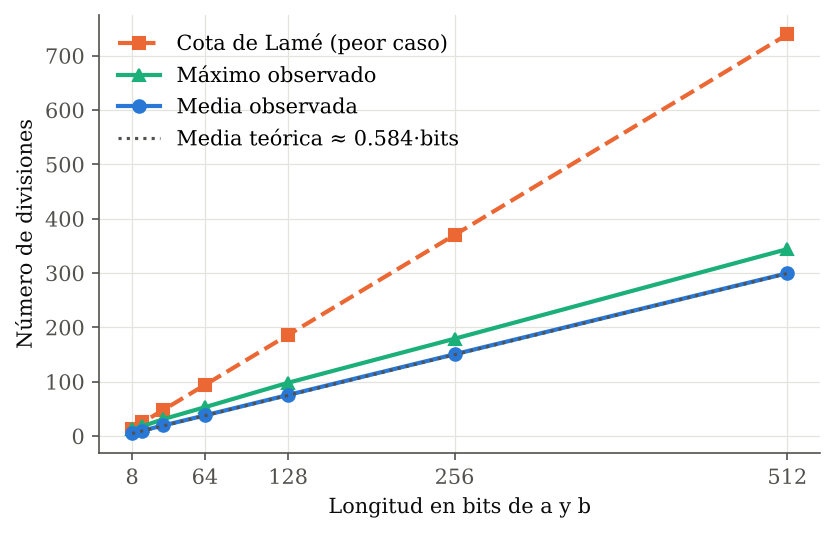
\includegraphics[width=0.75\textwidth, keepaspectratio]{fig1_euclides_divisiones.png}
    \caption{Divisiones del algoritmo de Euclides en función de la longitud en bits de la entrada}
    \label{fig:euclides_divisiones}
\end{figure}

\subsection{Escenario B: Exponenciación modular binaria rápida}
Se evaluaron exponentes de 8 a 1024 bits (256 casos en total). El Cuadro \ref{tab:potencia_operaciones} detalla el comportamiento del algoritmo instrumentado.

\begin{table}[H]
    \caption{Operaciones y latencia de la exponenciación binaria frente al tamaño del exponente}
    \label{tab:potencia_operaciones}
    \centering
    \scriptsize
    \begin{tabular*}{\textwidth}{@{\extracolsep{\fill}}cccccccc}
        \toprule
        Bits de $e$ & Cuadrados ($k-1$) & Productos (media) & Total mín. & Total medio & Total máx. & $\log_{10}(e-1)$ & Tiempo ($\mu$s) \\
        \midrule
        8    & 7     & 4.3   & 8    & 11.3   & 15   & 2.3   & 29.9 \\
        16   & 15    & 9.0   & 16   & 24.0   & 31   & 4.7   & 70.7 \\
        32   & 31    & 16.8  & 32   & 47.8   & 63   & 9.5   & 143.6 \\
        64   & 63    & 32.4  & 64   & 95.4   & 127  & 19.1  & 300.4 \\
        128  & 127   & 63.2  & 128  & 190.2  & 255  & 38.4  & 613.1 \\
        256  & 255   & 126.3 & 256  & 381.3  & 511  & 76.9  & 1\,221.3 \\
        512  & 511   & 252.9 & 512  & 763.9  & 1\,023 & 154.0 & 2\,572.6 \\
        1024 & 1\,023 & 510.7 & 1\,024 & 1\,533.7 & 2\,047 & 308.1 & 5\,016.4 \\
        \bottomrule
    \end{tabular*}
\end{table}

El número de cuadrados es exactamente $k - 1$ y los productos adicionales corresponden al peso de Hamming del exponente (con media $\approx k/2$). La Figura \ref{fig:potencia_operaciones} exhibe el crecimiento estrictamente lineal de las operaciones modulares.

\begin{figure}[H]
    \centering
    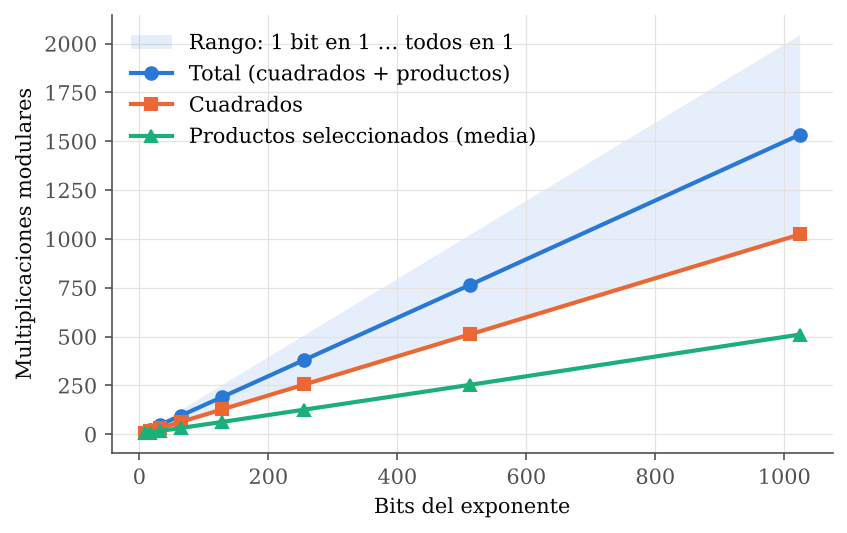
\includegraphics[width=0.75\textwidth, keepaspectratio]{fig2_potencia_operaciones.png}
    \caption{Desglose de operaciones de \texttt{modular\_pow}: cuadrados, productos y total}
    \label{fig:potencia_operaciones}
\end{figure}

\subsubsection{Comparación frente al método directo lineal}
El Cuadro \ref{tab:directo_vs_binario} y la Figura \ref{fig:directo_vs_binario} comparan la multiplicación iterativa directa frente a la exponenciación binaria. Para $e = 65\,535$ (16 bits), el método directo demandó 65\,534 multiplicaciones y $247.7$ ms, mientras que el binario requirió únicamente 31 operaciones y $0.099$ ms (aceleración de $2\,485\times$). Para $e$ de 1024 bits, el método directo requeriría del orden de $10^{308}$ operaciones, haciéndolo incomputable.

\begin{table}[H]
    \caption{Comparación entre el método directo iterativo y la exponenciación binaria}
    \label{tab:directo_vs_binario}
    \centering
    \footnotesize
    \begin{tabular*}{\textwidth}{@{\extracolsep{\fill}}ccccccc}
        \toprule
        $e$ & Bits ($k$) & Mult. directo ($e-1$) & Mult. binario & Tiempo directo ($\mu$s) & Tiempo binario ($\mu$s) & Aceleración \\
        \midrule
        255      & 8  & 254     & 15 & 1\,402.5   & 63.3 & $22.2\times$ \\
        4\,095   & 12 & 4\,094   & 23 & 20\,151.2  & 68.2 & $295.5\times$ \\
        65\,535  & 16 & 65\,534  & 31 & 247\,767.4 & 99.7 & $2\,485.2\times$ \\
        \bottomrule
    \end{tabular*}
\end{table}

\begin{figure}[H]
    \centering
    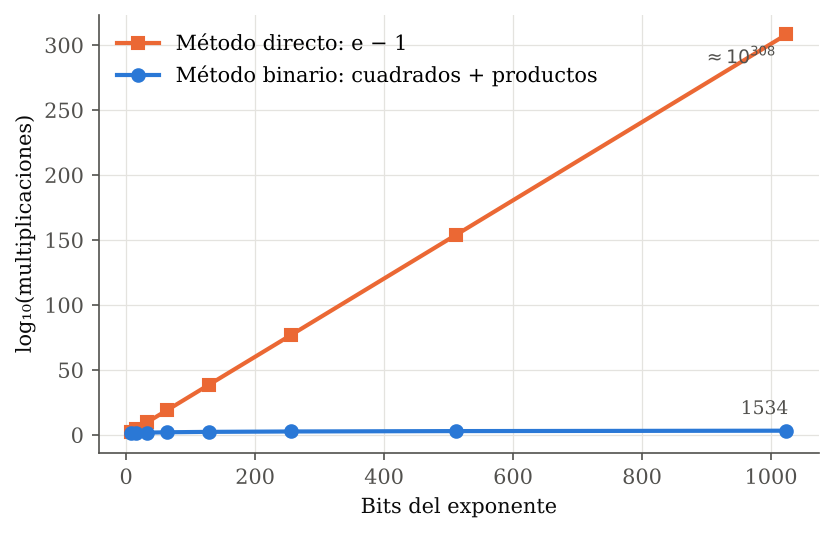
\includegraphics[width=0.72\textwidth, keepaspectratio]{fig3_directo_vs_binario.png}
    \caption{Crecimiento de multiplicaciones: método directo lineal vs. exponenciación binaria}
    \label{fig:directo_vs_binario}
\end{figure}

\subsubsection{Impacto del peso de Hamming en exponentes de 1024 bits}
Al fijar la longitud en $k = 1024$ bits y variar la cantidad de unos entre 1 y 1024, la latencia escala linealmente desde $3.4$ ms (para 1 solo producto, $e = 2^{1023}$) hasta $6.8$ ms (para 1024 productos, $e = 2^{1024}-1$), tal como refleja la Figura \ref{fig:unos_tiempo}.

\begin{figure}[H]
    \centering
    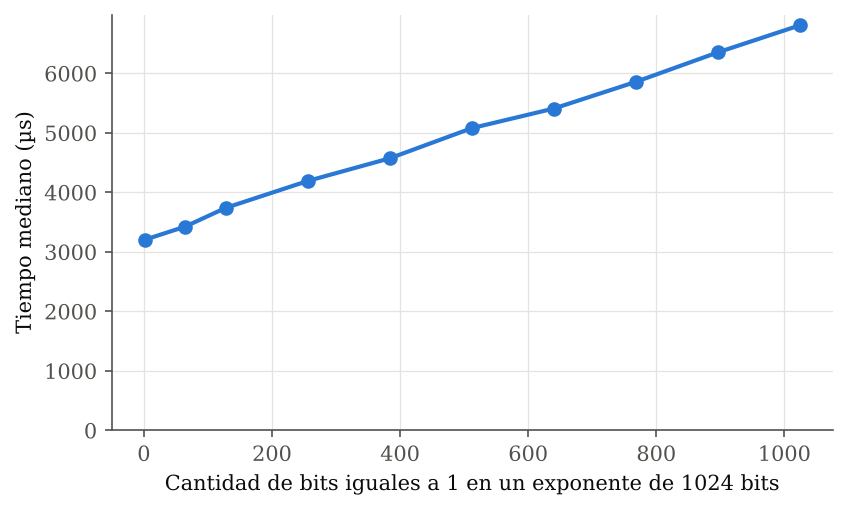
\includegraphics[width=0.72\textwidth, keepaspectratio]{fig4_unos_tiempo.png}
    \caption{Influencia del peso de Hamming sobre el tiempo de cómputo para $k = 1024$ bits}
    \label{fig:unos_tiempo}
\end{figure}

\subsection{Escenario C: Inversos modulares y congruencias lineales}
En 2\,000 evaluaciones de inverso modular, los 1\,209 casos con $\gcd(a, n) = 1$ generaron inversos válidos con $(a \cdot u) \bmod n = 1$, mientras que los 791 casos con $\gcd(a, n) > 1$ fueron interceptados con \texttt{ValueError} (Cuadro \ref{tab:inversos_ejemplos}).

\begin{table}[H]
    \caption{Casos representativos de evaluación de inversos modulares}
    \label{tab:inversos_ejemplos}
    \centering
    \footnotesize
    \begin{tabular*}{\textwidth}{@{\extracolsep{\fill}}ccccc}
        \toprule
        $a$ & $n$ & $\gcd(a, n)$ & Resultado & Verificación analítica \\
        \midrule
        7 & 40 & 1 & 23 & $(7 \cdot 23) \bmod 40 = 161 \bmod 40 = 1$ \\
        $-3$ & 11 & 1 & 7 & $(-3 \cdot 7) \bmod 11 = -21 \bmod 11 = 1$ \\
        17 & 3\,120 & 1 & 2\,753 & $(17 \cdot 2\,753) \bmod 3\,120 = 1$ \\
        6 & 9 & 3 & Rechazado & Lanza \texttt{ValueError} ($\gcd = 3 > 1$) \\
        10 & 25 & 5 & Rechazado & Lanza \texttt{ValueError} ($\gcd = 5 > 1$) \\
        14 & 100 & 2 & Rechazado & Lanza \texttt{ValueError} ($\gcd = 2 > 1$) \\
        \bottomrule
    \end{tabular*}
\end{table}

En 2\,000 congruencias lineales, el número de soluciones canónicas fue exactamente $d = \gcd(a, n)$ cuando $d \mid b$ y cero cuando $d \nmid b$ (Cuadro \ref{tab:congruencias_ejemplos}).

\begin{table}[H]
    \caption{Casos representativos de congruencias lineales y soluciones canónicas}
    \label{tab:congruencias_ejemplos}
    \centering
    \footnotesize
    \begin{tabular*}{\textwidth}{@{\extracolsep{\fill}}lcccc}
        \toprule
        \textbf{Congruencia evaluada} & $d = \gcd(a, n)$ & \textbf{Esperadas} & \textbf{Obtenidas} & \textbf{Conjunto de soluciones en $\mathbb{Z}_n$} \\
        \midrule
        $14x \equiv 30 \pmod{100}$ & 2 & 2 & 2 & $\{45, 95\}$ \\
        $6x \equiv 4 \pmod 9$      & 3 & 0 & 0 & $\emptyset$ (incompatible: $3 \nmid 4$) \\
        $7x \equiv 3 \pmod{40}$    & 1 & 1 & 1 & $\{29\}$ \\
        $12x \equiv 18 \pmod{30}$  & 6 & 6 & 6 & $\{4, 9, 14, 19, 24, 29\}$ \\
        $35x \equiv 10 \pmod{50}$  & 5 & 5 & 5 & $\{6, 16, 26, 36, 46\}$ \\
        \bottomrule
    \end{tabular*}
\end{table}
